\chapter{Supplementary figures}
\label{supplementaryfigures}

The next pages contain a list of supplementary figures providing additional insight on the approaches used to predict protein interactions using coevolution. All these figures are referenced in the main manuscript but relegated to the backend to improve the readability.

%%%%%%%%%%%%%%%%%%%%%%%%%%%%%%%%%%%%%%%%%%%%%%%%%%%%%%%%%%%%%%%%%%%%%%%%%%%%%%%%%%%%%%%%%%%%

\begin{figure}[htbp]
\centering
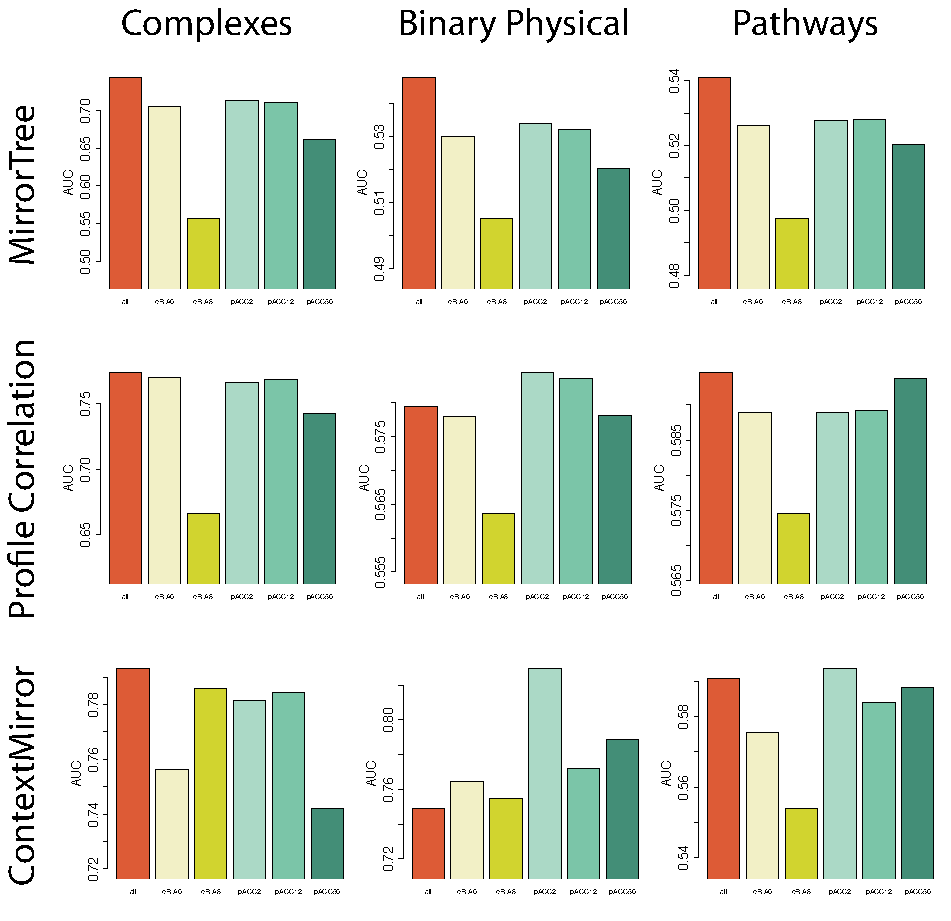
\includegraphics[keepaspectratio,width=\textwidth,height=0.75\textheight]{../figures/accsROCs_differentScales.pdf}
\caption{\textbf{Performance obtained using different combinations of: phylogenetic tree comparative methods, interaction evidence and predicted accessibility filter}. Different performances are calculated using the Area Under the ROC Curve (AUC). In order to highlight the differences between the different methods and interaction datasets, the scales were adjusted independently.}
\label{accsrocs_differentscales.pdf}
\end{figure}

\begin{figure}[htbp]
\centering
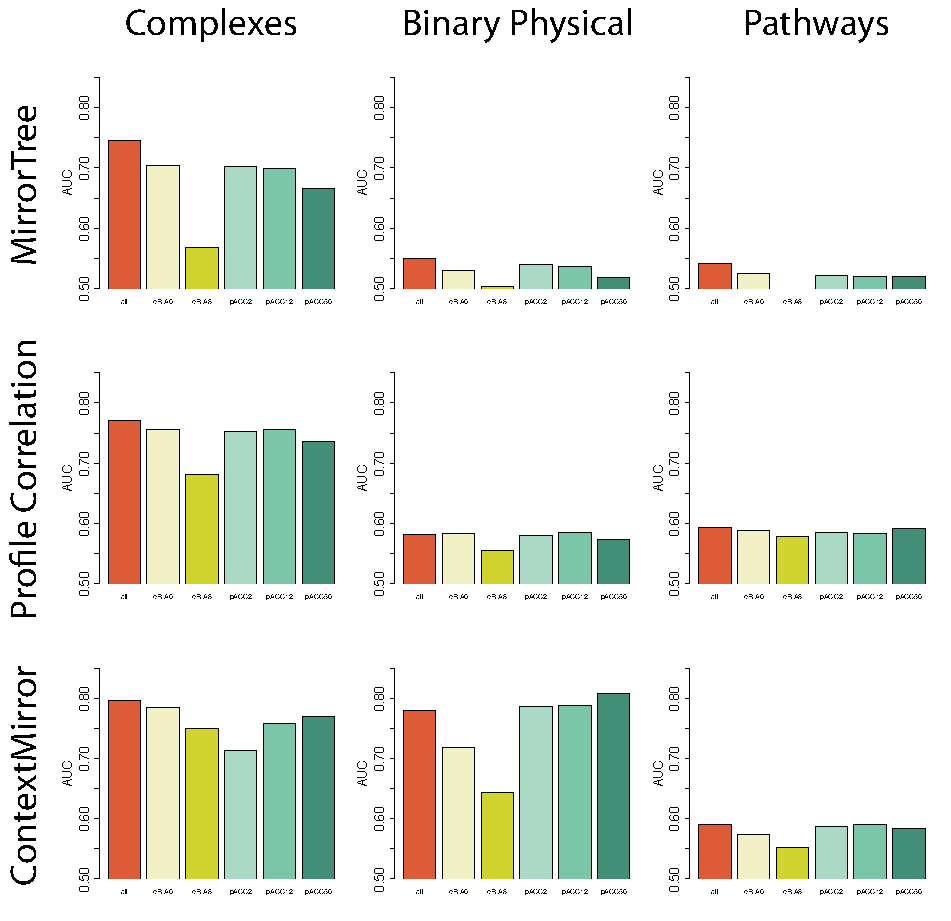
\includegraphics[keepaspectratio,width=\textwidth,height=0.75\textheight]{../figures/accsROCs_orthologs.pdf}
\caption{\textbf{Performances of the different methods predicting different types of interactions using trees derived from positions with different predicted accessibility features}. The performance is evaluated as the Area Under the ROC Curve (AUC) using predicted accessibility derived from MSAs of orthologs.}
\label{accsrocs_orthologs.pdf}
\end{figure}

\begin{figure}[htbp]
\centering
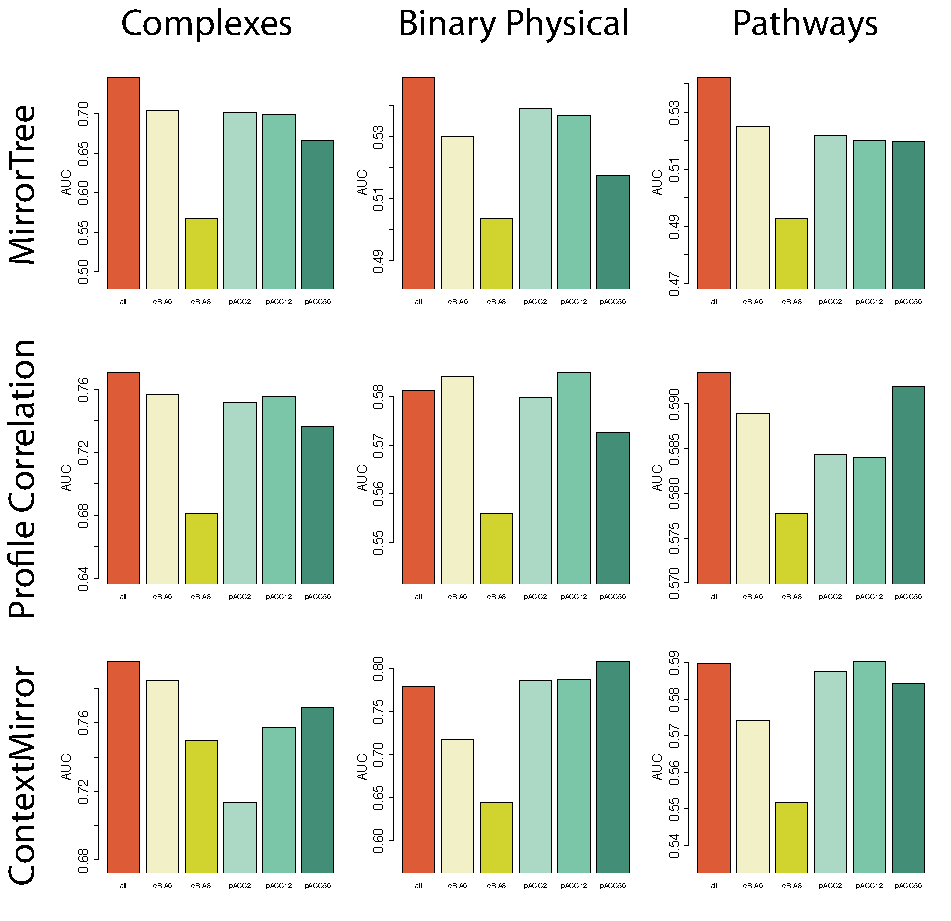
\includegraphics[keepaspectratio,width=\textwidth,height=0.75\textheight]{../figures/accsROCs_orthologs_scaled.pdf}
\caption{\textbf{Performances of the different methods predicting different types of interactions using trees derived from positions with different predicted accessibility features}. The performance is evaluated as the Area Under the ROC Curve (AUC) using predicted accessibility derived from MSAs of orthologs. In order to highlight the differences, the axis scales were adjusted independently for each case.}
\label{accsrocs_orthologs_scaled.pdf}
\end{figure}

\begin{figure}[htbp]
\centering
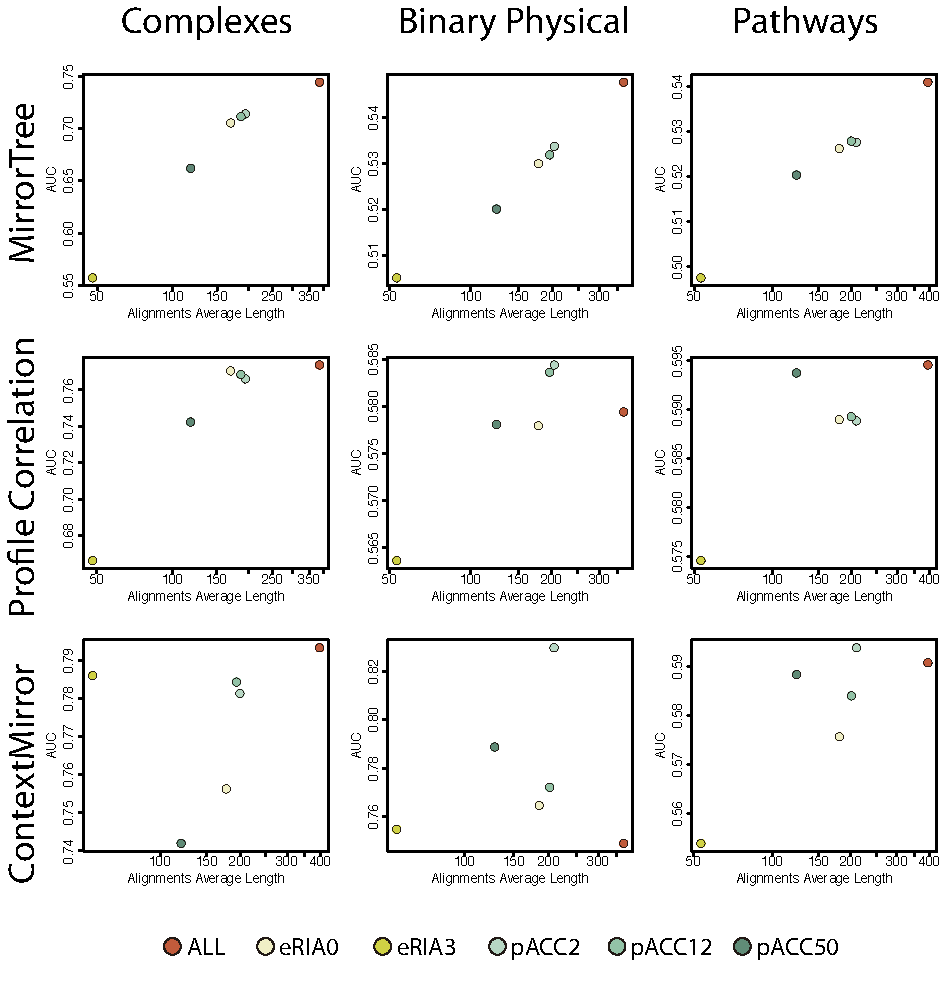
\includegraphics[keepaspectratio,width=\textwidth,height=0.75\textheight]{../figures/accsAlnLength_full.pdf}
\caption{\textbf{Relationship between the performances of the different methods and the lengths of the virtual alignments for the different datasets}. The length of the virtual alignment is the number of positions (fulfilling a given predicted accessibility criteria –colors-) used to construct the trees.}
\label{accsalnlength_full.pdf}
\end{figure}

\begin{figure}[htbp]
\centering
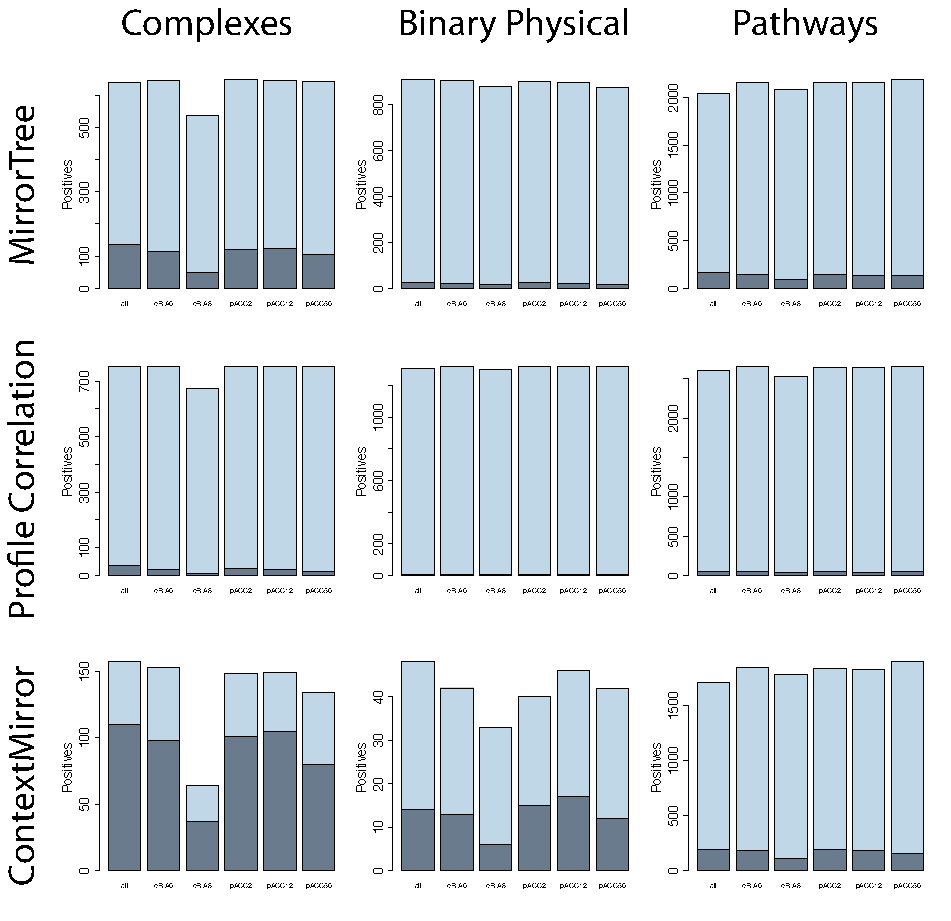
\includegraphics[keepaspectratio,width=\textwidth,height=0.75\textheight]{../figures/accsPositives.pdf}
\caption{\textbf{Positive predictions obtained using different combinations of: phylogenetic tree comparative methods, interaction evidence and predicted accessibility filter}. The bars represent the total number of positives (nP) for which the calculation could be done (fulfilling organisms in common and \emph{P}-value criteria) for a given prediction. The dark-blue bars, represent the subset of true positives among the first nP protein pairs.}
\label{accspositives.pdf}
\end{figure}

%%%%%%%%%%%%%%%%%%%%%%%%%%%%%%%%%%%%%%%%%%%%%%%%%%%%%%%%%%%%%%%%%%%%%%%%%%%%%%%%%%%%%%%

\begin{figure}[htbp]
\centering
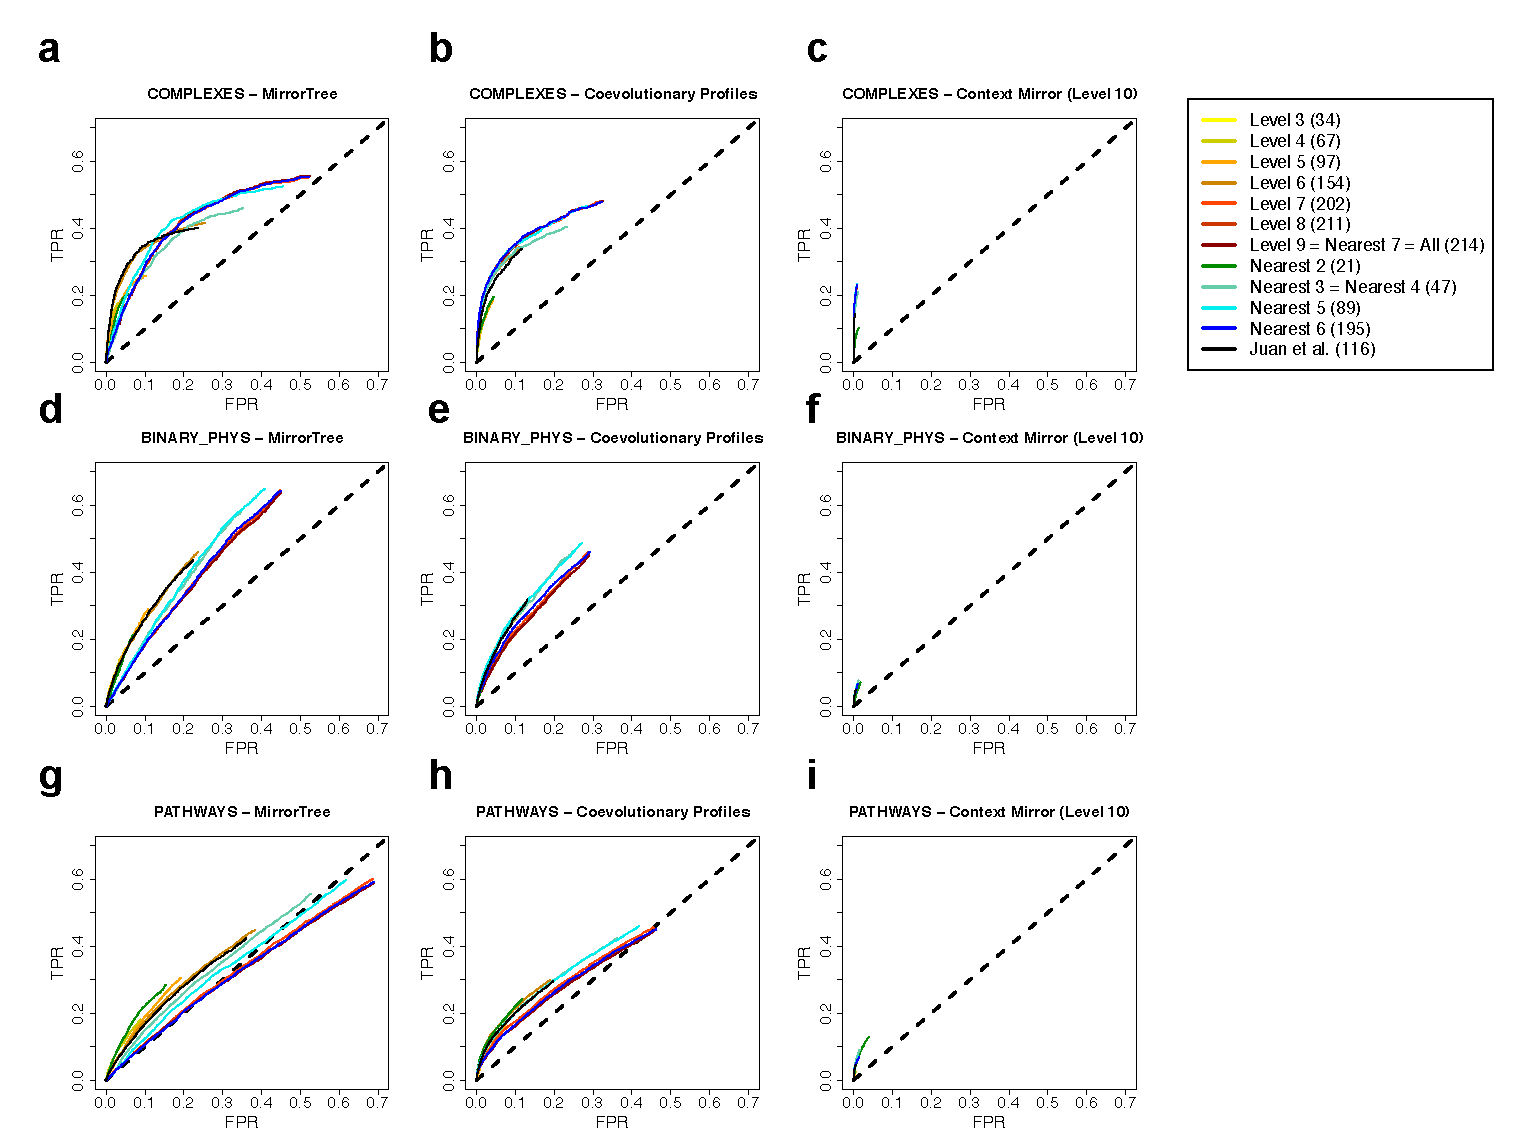
\includegraphics[keepaspectratio,width=\textwidth,height=0.75\textheight]{../figures/selectionROCs_noscales.pdf}
\caption{\textbf{Matrix of partial ROC curves}. The partial ROC curves evaluate the performance of a given list of predictions obtained by the combination of a methodology (columns), a dataset of interactions (rows) and a set of organisms (colors according to the legend). In the legend, the number of organisms present in the dataset is included within brackets. The dashed line represents the performance of a random classifier. The different plots are in the same scale in order to compare their global performances.}
\label{selectionrocs_noscales.pdf}
\end{figure}

\begin{figure}[htbp]
\centering
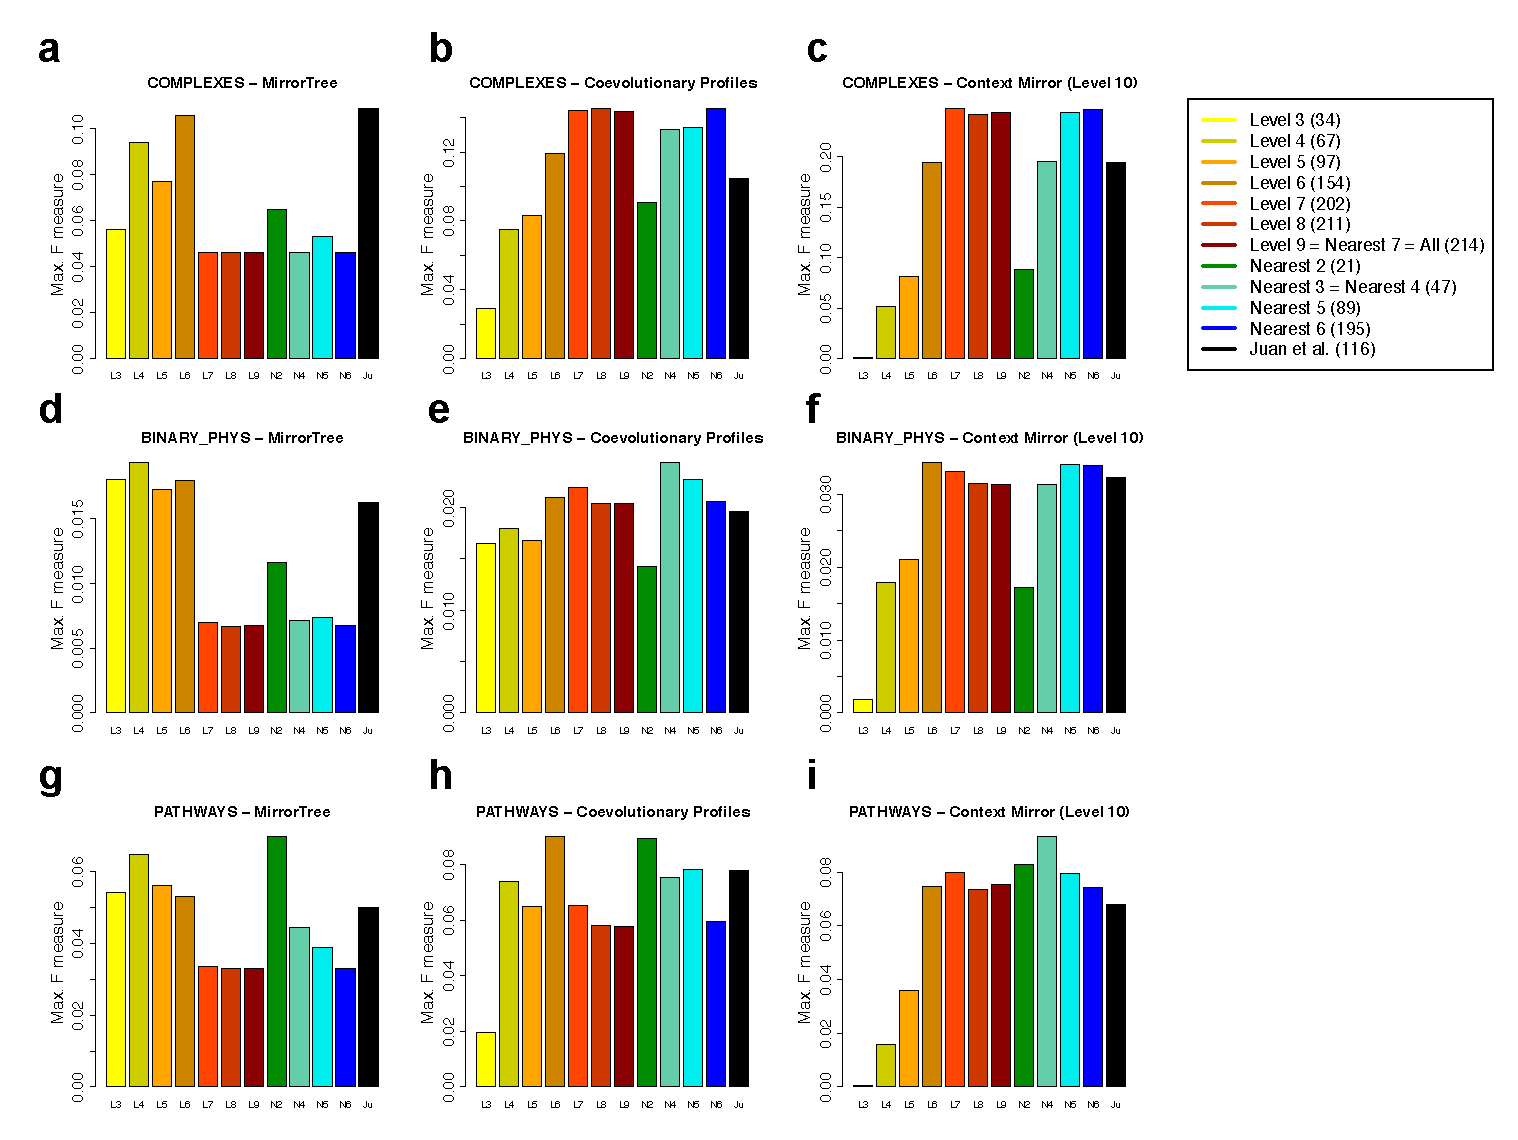
\includegraphics[keepaspectratio,width=\textwidth,height=0.75\textheight]{../figures/selectionMaxFmeasure.pdf}
\caption{\textbf{Maximum F-measure for each method\slash organism set}. The optimal F-measure along the range of possible cutoffs is showed in these bar plots. The rows represent the interaction dataset and the columns the methods. For a given combination of method and interaction dataset the colored bars represent different sets of organisms used to reconstruct the phylogenetic trees. Extended labels, as well as the number of organisms are shown in the legend.}
\label{selectionmaxfmeasure.pdf}
\end{figure}

%%%%%%%%%%%%%%%%%%%%%%%%%%%%%%%%%%%%%%%%%%%%%%%%%%%%%%%%%%%%%%%%%%%%%%%%%%%%%%%%%%%%%%%

\begin{figure}[htbp]
\centering
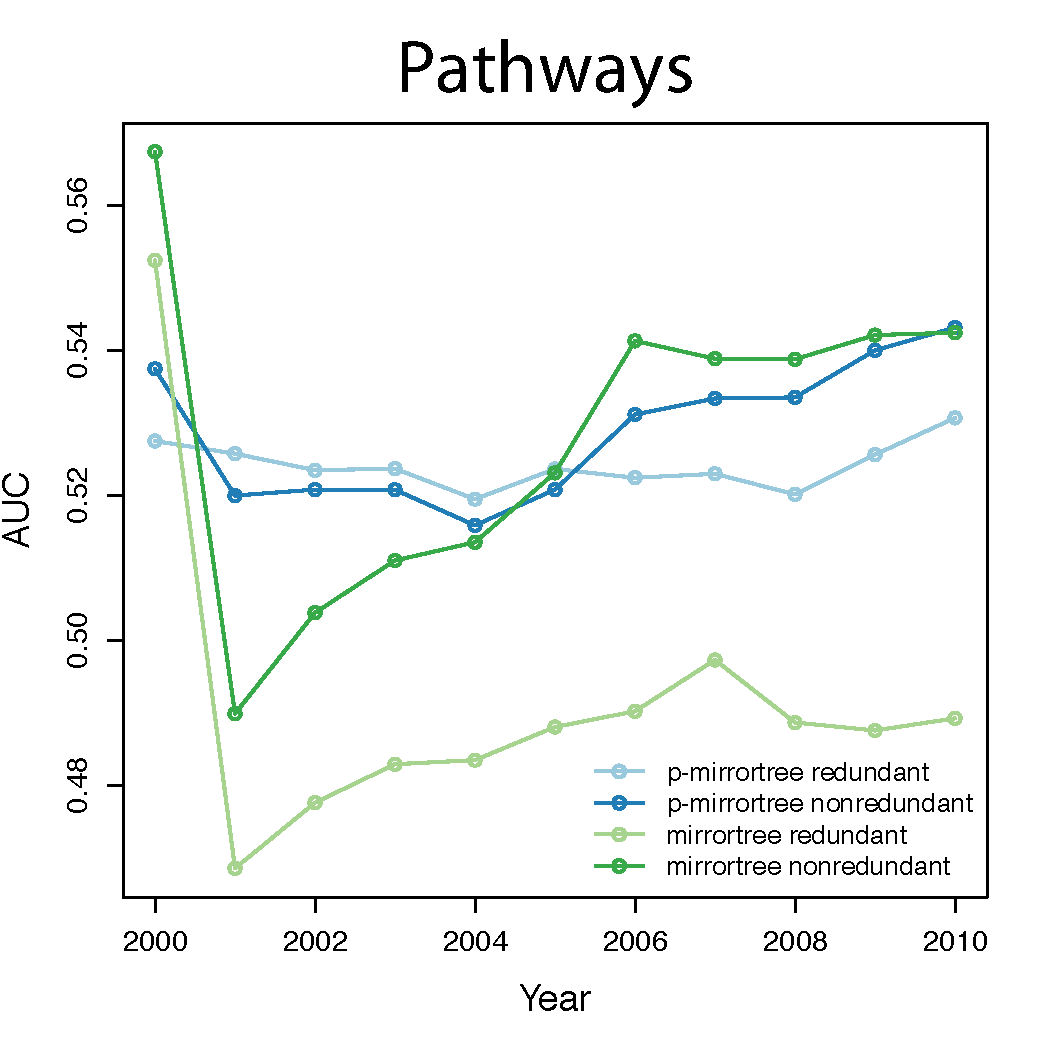
\includegraphics[keepaspectratio,width=\textwidth,height=0.75\textheight]{../figures/mthistoric_pthwys.pdf}
\caption{\textbf{Performance of the \emph{mirrortree} and \emph{p-mirrortree} methods when predicting interactions using different sets of organisms based on the fully-sequenced genomes available in the period 2000-2010 and different taxonomical redundancies}. The performances were evaluated in terms of AUC using a gold standard dataset of protein interactions defined as co-membership in the same KEGG pathway.}
\label{mthistoric_pthwys.pdf}
\end{figure}

\begin{figure}[htbp]
\centering
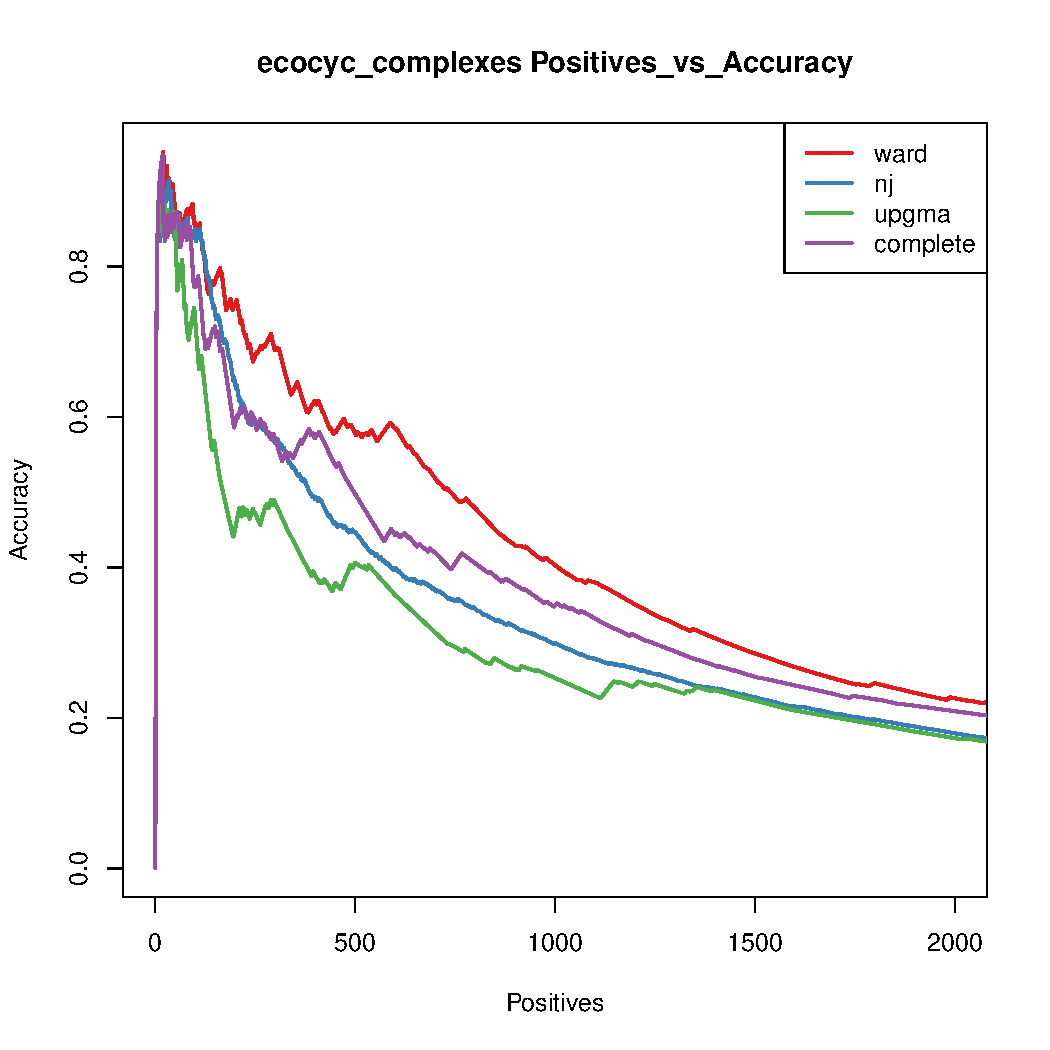
\includegraphics[keepaspectratio,width=\textwidth,height=0.75\textheight]{../figures/mtclustering_methods.pdf}
	\caption{\textbf{Accuracy \emph{vs.} number of positives in 4 different hierarchichal clustering algorithms predicting protein interactions}. Cophenetic distances from the resulting clustering of coevolutionary profiles were used to score the predictions. The clusterings algorithms were based on Ward's minimum variance (``ward''), neighbor-joining (``nj''), UPGMA (``upgma'') and complete linkage (``complete''). Protein interactions were evaluated using the ``Complexes'' gold standard dataset.}
\label{mtclustering_methods.pdf}
\end{figure}